\chapter{Adaptaci'on}
\label{capitulocuatro}

\section{Adaptaci'on transparente y transformaci'on operacional}

Los sistemas groupware en tiempo real son construidos generalmente guiados por uno de los siguientes enfoques: conciencia de colaboración (collaboration awareness) y transparencia de colaboraci'on (collaboration transparency).
\medskip
Con el primer enfoque los groupware son desarrollados especialmente con el prop'osito de soportar la colaboraci'on y con mecanismos internos de conciencia de colaboraci'on desde su dise'no. Con el segundo enfoque, los groupware que est'an basados en sistemas existentes o nuevos, presentan mecanismos externos que no fueron pensados en el dise'no. [Qian Xia, 2006].
\medskip
Una ventaja de la colaboración transparente es que permite a los usuarios realizar colaboraciones con las aplicaciones que le son familiares, “¿Qui'en abandonaria su editor de texto favorito para usar una aplicaci'on de autoria colaborativa? - Who would abandon their favorite word processors to use a co-authorship application?” [Grudin, 1994 b], asimismo el agregar funcionalidades de colaboración en aplicaciones mono-usuario reduce el esfuerzo de desarrollar groupwares.

\section{Adaptaci'on Transparente}

A diferencia de otras t'ecnicas de transformaci'on de aplicaciones en aplicaciones compartidas, la adaptación transparente (TA) intenta transformar de forma transparente una aplicaci'on mono-usuario en una versión colaborativa del mismo, en el caso espec'ifico del proyecto, se trabaj'o 'unicamente con ambientes homog'eneos, lo cual significa que se requiere el uso de la misma aplicaci'on convertida en las sesiones de colaboraci'on.
\medskip
En los fundamentos de la adaptaci'on transparente, se trabaja con la API (Application Programming Interface - Interfaz de programaci'on de la aplicaci'on) para de esta manera interceptar las acciones realizadas por los usuarios y asi sin modificar el c'odigo
fuente de la aplicaci'on permitir la comunicaci'on del sistema mono usuario con los dem'as miembros de la sesi'on.
\medskip
El proyecto sobre el que se trabaj'o no cuenta con una API como tal, para poder realizar la intercepci'on de los eventos, pero tras analizar la estructura del proyecto, se identificaron las
operaciones claves a interceptar, es en este momento en el que se decidi'o usar herramientas de la Transformaci'on Operacional (OT) para manipular e interceptar los eventos generados, en este caso modificando levemente el manejo de los eventos dentro de la aplicaci'on de tipo mono usuario.

\medskip

El n'ucleo de la aplicaci'on de dise'no de interfaces se centra en tres acciones fundamentales:

\begin{itemize}
\item Agregar componente.
\item Editar componente.
\item Eliminar componente.
\end{itemize}

\medskip
Para poder llevar a cabo una adaptaci'on transparente como tal se pide poner especial 'enfasis en los siguientes puntos:
\medskip
\paragraph{Compatibilidad de la aplicaci'on​:}
Las caracter'isticas y funcionalidades de la interfaz de usuario as'i como los formatos de los documentos deben ser mantenidos.

\paragraph{Transparencia de la aplicaci'on:}
​No se deben realizar cambios al c'odigo original de la aplicaci'on en lo posible. Esta caracter'istica no pudo ser completada a falta de una forma de comunicaci'on con la aplicaci'on sobre la que se realiza el trabajo, por lo que se hizo 'enfasis en modificar lo m'inimo necesario para poder realizar la transformaci'on de la manera m'as transparente posible.

\paragraph{Respuesta local rapida:}
​La respuesta del sistema una vez modificado debe ser lo m'as parecida a la versi'on original. Para poder mantener esta caracter'istica puesto que como enfoque se escogi'o una arquitectura centralizada, se restringe que los miembros del equipo se encuentren de momento sobre la misma red.

\paragraph{Colaboraci'on sin restricciones:}
Los usuarios deben ser libres de realizar la mayor cantidad de operaciones con los datos en cualquier momento, lo que implica un
WYSIWIS (What you see is what I see - Lo que ves es lo que veo) relajado y trabajo concurrente. En un ambiente de WYSIWIS estricto, todos los integrantes del grupo de trabajo tienen que estar
estrictamente viendo lo mismo en un mismo ambiente. En cambio en un ambiente de WYSIWIS relajado si bien los integrantes se encuentran sobre un mismo sistema, presentan la libertad de moverse y realizar acciones diferentes a las de sus compa'neros de piso.

\paragraph{Conciencia de espacio de trabajo:}
​El sistema deberá soportar una variedad de
características de conciencia de espacio de trabajo, para permitir a los usuarios
conocer quien está trabajando con ellos y que están realizando.

\section{Modelo de adaptaci'on}

Para comenzar con la adaptación del sistema, se utilizo  el sistema para identificar las acciones fundamentales ya descritas, existen diferentes formas de realizar una misma acci'on dentro del sistema, y revisando la estructura de la forma en la que se manejan los eventos de los usuarios, se detect'o que una misma acci'on realizada desde diferentes lugares dentro de la aplicaci'on se traducen en diferentes acciones dentro de la misma \ref{fig:FV}, por lo que para comenzar con la transformaci'on del proyecto primero se dio paso a una ligera refactorizaci'on del sistema.

\begin{figure}[h]
    \centering
    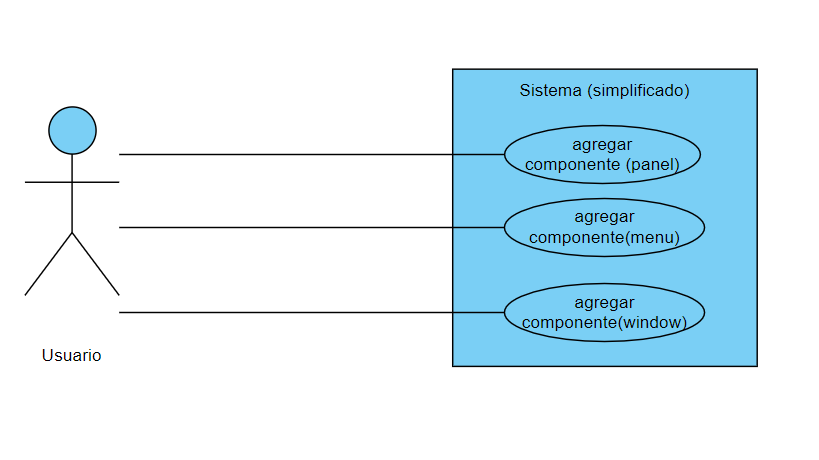
\includegraphics[width=0.55\textwidth]{Figura0401FirstView}
    \caption{Estado inicial del sistema, ejemplo.}
    \label{fig:FV}
\end{figure}




%
%\section{Motivaci'on}
%
%Para realizar el experimento se utiliz'o dos tipos de datos: contribuci'on a clases e interacci'on de clases; por las siguientes razones:
%
%\begin{itemize}
%\item \emph{Contribuciones a clases}. Cuando un conjunto de personas se reune para desarrollar software, tienden a trabajar juntos, por lo tanto la mayoria de las clases dentro de un proyecto son trabajadas por varias personas. Entender que personas trabajaron sobre ciertas clases, en ciertos periodos de tiempo ayuda a conocer el trabajo de cada contribuidor, que personas trabajaron en conjunto, que clases fueron modificadas en determinados tiempos, etc.\cite{Fritz}
%\item \emph{Interacci'on entre clases}. Al programar en el paradigma orientado a objetos, se hace uso de lo que es envio de mensajes o llamadas de m'etodos. Durante la ejecuci'on del programa, los objetos que son creados se mandan mensajes unos a otros. Entender entre que clases y en que momento se realiza este paso de mensajes ayuda a la optimizaci'on del software.\cite{Sillito}
%\end{itemize}
%
%\section{Conjunto de datos}
%
%Los dos conjuntos de datos utilizados para el experimento se escogieron a partir de las motivaciones anteriormente mencionadas, son datos reales del entorno de Pharo, recopilados en archivos .csv y se describen a continuaci'on:
%\begin{itemize}
%\item \emph{Contribuciones a clases}. Este conjunto de datos trata de las contribuciones realizadas sobre clases del modulo Trachel durante alg'un tiempo y los pesos representan la cantidad de l'ineas modificadas por un contribuidor en una clase. \\
%Trachel es un API (Application Programming Interface) de bajo nivel que permite dibujar elementos gr'aficos en Pharo, en la figura \ref{fig:Trachel} inciso a). se muestra el paquete de Trachel en el navegador de Pharo. Trachel esta compuesto por 5 elementos: contenedores gr'aficos (Canvas), figuras (Shape), eventos (Event), una entidad para enfocar porciones de contenedores (Camera) y ofrece animaci'on sobre figuras (Viva). \\
%Los datos est'an recopilados en el archivo Trachel.csv y se deduce que los datos fueron recopilados durante un periodo corto dado que s'olo se encuentra en el archivo 10 tiempos distintos. 'Este archivo contiene 525 tuplas en total, se distinguen a 22 contribuidores distintos y 98 clases del modulo Trachel.
%Por lo tanto en t'erminos de MultiPile Matrix el archivo Trachel.csv se representa en 10 matrices (tiempos) cada una de una tama'no de \textbar~22 x 98 \textbar.
%
%\begin{figure}[h]
%    \centering
%    \includegraphics[width=1\textwidth]{Figura0401Trachel}
%    \caption{En el inciso a). esta el paquete de Trachel y en el inciso b). algunas clases de Roassal ambos en el navegador de Pharo. Fuente: \url{http://pharo.org/}}
%    \label{fig:Trachel}
%\end{figure}
%
%\item \emph{Interacci'on entre clases}. Este conjunto de datos trata de como una clase del modulo de Roassal en tiempo de ejecuci'on interactua con otra, los pesos solo pueden ser dos valores 0 'o 1; es decir, tiene interacci'on o no. \\
%Roassal es el motor visual de Pharo, es utilizado para graficar elementos, en la figura \ref{fig:Trachel} inciso b). se muestra algunas de las clases de Roassal en el navegador de Pharo. Se desconoce el pedazo de c'odigo que se ejecuto para sacar los datos necesarios en el archivo resultante ClassDep04.csv. \\
%ClassDep04.csv contiene 643 tuplas en total, en 'este archivo se distinguen 19 tiempos distintos, con 26 clases distintas que mandan mensajes y 32 clases distintas que reciben mensajes.
%Por lo tanto en t'erminos de MultiPile Matrix el archivo ClassDep04.csv se muestra como 19 matrices (tiempos) cada una de una tama'no de \textbar~26 x 32 \textbar.
%\end{itemize}
%
%\section{Herramienta para comparar}
%Se opta por MS-Excel porque es una herramienta que se utiliza por defecto para manipular datos tabulares. Ofrece una larga lista de operaciones para manipular datos: filtros, ordenamiento, transformaciones, creaci'on de gr'aficos y definici'on de macros. Tambi'en excel tiene la ventaja de ser conocido por una gran poblaci'on y fue utilizado para muchos experimentos similares\cite{Cube14}.
%
%\section{Evaluaci'on}
%Esta evaluaci'on realiza una observaci'on sobre dos aspectos uno de ellos es el lenguaje, la primera es saber si el DSL es 'util; para ello se tiene la pregunta Q1 - ``?`Cu'an importantes son las caracter'isticas ofrecidas por MultiPile Matrix DSL para responder?''. El segundo aspecto es si esta visualizaci'on reduce el tiempo e incrementa la exactitud de las consultas, para ello se tiene la pregunta Q2 - ``?`Cu'an efectivo es MultiPile Matrix contra la herramienta est'andar?''.
%
%\section{Dise'no del experimento}
%Para realizar la evaluaci'on del proyecto se necesito de material, estrategia y participantes. El material que se dispuso para el experimento consiste de:
%\begin{itemize}
%\item \emph{Material de aprendizaje de Excel}: Este material de aprendizaje provee un imagen que resume las funciones que Excel ofrece para ordenar y filtrar. Para mayor informaci'on ver el anexo \ref{MaterialExcel}.
%\item \emph{Material de aprendizaje de MultiPile Matrix}: Se provee una descripci'on de las partes de MultiPile, las funcionalidades que ofrece acompa\~{n}adas de im'agenes. Es un resumen de la secci'on \ref{Aplicaciones}. Para mayor informaci'on ver el anexo \ref{MaterialMM}.
%\item \emph{Tarea 1}: Consiste en contestar con ayuda de alguna herramienta (MultiPile Matrix o Excel) a un cuestionario de 5 preguntas para el conjunto de datos referente a la contribuci'on de clases plasmado en el archivo Trachel.csv.
%\item \emph{Tarea 2}: Consiste en contestar con ayuda de alguna herramienta (MultiPile Matrix o Excel) a un cuestionario de 5 preguntas para el conjunto de datos referente a la interacci'on de clases plasmado en el archivo ClassDep04.csv.
%\item \emph{Retrospectiva}: Se pide la opini'on del participante de manera verbal para conocer la impresi'on que tuvo de la herramienta.
%\end{itemize}
%
%La estrategia consiste en la asignaci'on de las tareas entre los participantes, como se observa en la tabla \ref{tab:Tabla4.1}; tambi'en para que el ambiente sea lo m'as controlado posible, se realizo el experimento participante por participante en la misma maquina, de tal manera que se tienen 4 participantes para cada tarea con cada una de las herramientas.
%
%\begin{table}[h]
%\centering
%\begin{tabular}{l|l|l}
%\textbf{Participante} & \textbf{Tarea 1} & \textbf{Tarea 2} \\ \hline
%P1                    & EX               & MM               \\ \hline
%P2                    & MM               & EX               \\ \hline
%P3                    & EX               & MM               \\ \hline
%P4                    & MM               & EX               \\ \hline
%P5                    & EX               & MM               \\ \hline
%P6                    & MM               & EX               \\ \hline
%P7                    & EX               & MM               \\ \hline
%P8                    & MM               & EX               \\ \hline
%\end{tabular}
%\caption{Asignaci'on de herramientas y tareas. Fuente: Elaboraci'on propia}
%\label{tab:Tabla4.1}
%\end{table}
%
%A continuaci'on se describen las tareas que se crearon para el experimento. Para la Tarea 1 (Trachel.csv) se tienen las siguientes 5 preguntas: 
%\begin{itemize}
%\item Q1 - ?`Cu'al es la mayor cantidad de clases modificadas por un sola persona en un solo periodo entre los primeros cuatro periodos y quien fue?
%\item Q2 - ?`Qu'e contribuidores no realizaron cambios en clases del intervalo [2 - 8]?
%\item Q3 - ?`Qu'e clases fueron modificadas en cada tiempo durante todo el proyecto?
%\item Q4 - ?`Qu'e clases no fueron modificadas en el intervalo de tiempo donde TRArcShape fue modificado?
%\item Q5 - ?`Qu'e contribuidor no realizo cambios en el intervalo de tiempo donde TRCompositeShape fue modificado?
%\end{itemize}
%
%La 'unica pregunta que tiene como respuesta un dato es Q5, las dem'as son preguntas en las cuales se requiere identificar m'as de una clase o m'as de un contribuidor o m'as de un dato.
%
%Para la Tarea 2 (ClassDep04.csv) se tienen las siguientes preguntas:
%\begin{itemize}
%\item Q1 - ?`Qu'e clases no mandaron mensajes durante los 'ultimos cuatro tiempos?
%\item Q2 - ?`Qu'e par de clases (C1, C2, 1) interactuan en cada tiempo que pertenece al intervalo [1 - 3]?
%\item Q3 - ?`Qu'e clases reciben mensajes solo en el ultimo tiempo?
%\item Q4 - ?`Qu'e clases reciben mensajes en cada tiempo en el intervalo donde RTMapExample mando o recibio mensajes?
%\item Q5 - ?`Qu'e clases no mandaron mensajes en el intervalo donde RTPopup mando o recibio mensajes?
%\end{itemize}
%
%Para todas las preguntas se requiere identificar un conjunto de clases o pares de clases.
%
%\section{Modo de calificaci'on}
%\label{sec:cali}
%Un participante puede responder a las preguntas con las respuestas que crea correctas. Este experimento se basa en la puntuaci'on de F-Measure o Valor-F, esta medida es una combinaci'on de la precisi'on y el recall. Para cada pregunta se calific'o de la siguiente forma: 
%\begin{itemize}
%\item \emph{Precisi'on}. Est'a dada por la cantidad de respuestas correctas relacionadas divido entre la cantidad de respuestas seleccionadas; es decir: $RCS/RS$.
%\item \emph{Recall}. Est'a dado por la cantidad de respuestas correctas relacionadas divido entre la cantidad de respuestas correctas; es decir: $RCS/RC$.
%\end{itemize}
%La puntuaci'on para cada pregunta se encuentra entre 0 y 1.
%Para cada tarea se tiene en cuenta la precisi'on y el recall, la nota de un participante en recall $x$ est'a dada por: \\* $PR(x) = \sum_{n=1}^5 PuntuacionRecall(Q_n, x)$ y en precisi'on por:
%\\* $PP(x) = \sum_{n=1}^5 PuntuacionPrecision(Q_n, x)$. Ambas puntuaciones se encuentran entre 0 y 5. Siendo 5 la mayor puntuaci'on posible.
%
%El F-Measure de cada participante esta dado por $P(x) = 2 * (PP(x) * PR(x)) / (PP(x) + PR(x))$. Tambi'en 'esta puntuaci'on se encuentra entre 0 y 5.
%
%\section{Estudio piloto}
%Antes de realizar todo el experimento, se realizo un estudio piloto con dos personas de la Universidad de Santiago de Chile, ambos finalizan estudios de maestria en ciencias de la computaci'on. Tambi'en ambos conocen Pharo y manejan Excel durante m'as de 5 a'nos. Este estudio ayudo a observar algunos puntos del experimento como:
%
%\begin{itemize}
%\item Ambas tareas se pueden realizar con Excel y MultiPile Matrix.
%\item Ambos participantes tuvieron la necesidad de observar documentaci'on sobre Excel. Se opto como conveniente que los participantes recurran a busquedas en internet sobre Excel como ayuda para el experimento.
%\item El material de aprendizaje de MultiPile Matrix se modifico con algunas observaciones de parte de los participantes de piloto.
%\item El cuestionario original tenia preguntas ambiguas o no claras, entonces se analizo y mejoro el cuestionario. 
%\end{itemize}
%
%El anexo \ref{MaterialMM} ofrece mayor informaci'on del estudio piloto.  
%
%\section{Resultados}
%Se realizo el experimento con 8 participantes de los cuales se puede destacar las siguientes caracter'isticas: todos tenian experiencia de minimamente 4 a'nos con Excel, todos conocian el paradigma OO y programaron en 'el, pero ninguno tenia conocimiento de Pharo. Entre estos participantes se encuentran 3 profesionales en ingenier'ia inform'atica, 3 estudiantes no graduados realizando su tesis en ingenier'ia inform'atica o de sistemas y 2 estudiantes no graduados entre sexto semestre y noveno semestre de las carreras de ingenier'ia inform'atica o de sistemas.
%
%\begin{figure}[h]
%    \centering
%    \includegraphics[width=0.55\textwidth]{Figura0402RE}
%    \caption{Resultado de la precisi'on y recall del experimento y las puntuaciones de Excel resaltadas con gris. Fuente: Elaboraci'on propia}
%    \label{fig:RE}
%\end{figure}
%
%En la figura \ref{fig:RE} se muestran los resultados de precisi'on y recall de cada participante, la primera columna tiene los identificadores de los participantes. Las siguientes 10 columnas muestran la puntuaci'on para cada pregunta de la tarea 1 y luego de la tarea 2.
%
%Las 'ultimas dos columnas son la puntuaci'on total mencionada en la secci'on \ref{sec:cali} para Excel y MultiPile Matrix. Las puntuaciones para Excel estan resaltadas en gris para una lectura m'as comprensible. 
%
%\begin{figure}[h]
%    \centering
%    \includegraphics[width=0.75\textwidth]{Figura0403RT}
%    \caption{Resultado del Valor-F de cada participante en el experimento y en la parte izquierda los tiempos que se demor'o cada participante. Fuente: Elaboraci'on propia}
%    \label{fig:RT}
%\end{figure}
%
%Mientras que en la figura \ref{fig:RT} la tabla de la parte derecha muestra las puntuaciones de cada participante del Valor-F, criterio en el que este experimento se basa. Y en la tabla izquierda se presenta el tiempo que tardo cada participante al realizar la tarea 1 y la tarea 2, este tiempo esta en minutos. Nuevamente las puntuaciones para Excel estan resaltadas en gris. 
%
%\begin{figure}[h]
%    \centering
%    \includegraphics[width=0.4\textwidth]{Figura0404Box}
%    \caption{Resultado del an'alisis del Valor-F. Fuente: Elaboraci'on propia}
%    \label{fig:Box}
%\end{figure}
%
%Para el an'alisis de los resultados se realizo la figura \ref{fig:Box} que a simple vista muestra que MultiPile Matrix tiene un efecto positivo tanto en precision como en recall. En la misma figura se muestra el an'alisis de los resultados de Valor-F, en la cual MultiPile Matrix sigue manteniendo un efecto positivo, con una m'axima puntuaci'on de 5, una m'inima de 4.5 y la media de $4.875 \pm 0.0590$, mientras que con Excel una m'axima de 4.6, una m'inima de 1.78 y la media de $3.448 \pm 0.2863$. 
%
%Para demostrar que los resultados no son a favor de la herramienta por suerte, se realizaron los siguientes pasos:
%
%\begin{itemize}
%\item El primer paso es formular una hipotesis nula, en este caso la hipotesis nula es: La puntuaci'on de MultiPile Matrix no es diferente a la de Excel. 
%\item El segundo paso es tratar de rechazar la hipotesis nula. Para rechazarla se realiza primero un test de normalidad, en este caso se uso ``Shapiro-Wilk normality test'' \cite{test}, 'este test verifica si los resultados son parte de una poblaci'on distribuida normalmente; este test tiene condiciones sobre los valores para ser considerado una opci'on para rechazar la hipotesis nula. Debido a la cantidad de datos y a su valor se encuentra que los datos de MultiPile Matrix no son normales y esa es una condici'on para continuar con este test.
%\item Ya que los datos no son normales se utilizo ``Mann-Whitney test'' \cite{test}, 'este test trabaja con valores no normales e indica si hay una diferencia significativa entre los resultados de Excel y MultiPile Matrix. Se considera que hay una diferencia significativa o que la hipotesis nula es rechazada, cuando el valor $P$ del calculo del test es menor a 0.05.
%\end{itemize}
%
%Una vez realizado el ``Mann-Whitney test''($P<0.05$) teniendo un $P = 0.0005$, que indica que la diferencia entre los resultados de Excel y MultiPile Matrix es significativa.
%
%Por lo tanto en este experimento se aprecia que:
%\begin{itemize}
%\item Los participantes consiguieron puntuaciones mejores y significativas usando MultiPile Matrix que con Excel.
%\item Los participantes completaron el cuestionario mucho m'as r'apido usando MultiPile Matrix que con Excel.
%\end{itemize}
%
%\section{Uso de Excel}
%Se observo a cada participante a medida que respondia las preguntas con Excel, 3 participantes recurrieron a ayuda online acerca de las funciones para quedarse con datos 'unicos, 5 participantes usaron distintas funciones de Excel, por ejemplo la funci'on COUNTIF, SUMIF, o agregando columnas extras, teniendo as'i un mejor tiempo que los dem'as participantes. 
%Se debe resaltar que no existe alguna pregunta en la que todos los participantes tuvieran el puntaje m'aximo. Y que el participante P8 fue el que mejor nota obtuvo, pero solo utilizo funciones de ordenamiento, filtros y filtros 'unicos.
%
%\section{Uso de MultiPile Matrix}
%Al observar los usos de MultiPile Matrix, fue sorprendente notar que no utilizaron todas las caracter'isticas del material de aprendizaje. Si bien en las primeras preguntas de ambas tareas se debia realizar una apilaci'on de un intervalo, los participantes P2 y P3 solo vieron necesario ver el timeLine para responder. Los participantes P5 y P4 a medida que realizaban una apilaci'on por criterio tambi'en resaltaban las relaciones que satisfacian el mismo criterio. Para la Q2 de la tarea 2 todos los participantes utilizaron el resaltado de peso, obteniendo respuestas correctas con MultiPile Matrix. Para la tarea 1, las preguntas Q2, Q3 y Q5 tuvieron respuestas correctas para todos los participantes, utilizando las opciones de apilaci'on y observando las partes que componen una pila. Para la tarea 2, las preguntas Q1, Q2, Q4 y Q5 tuvieron respuestas correctas para todos los participantes, utilizando resaltado y opciones de apilaci'on.
%
%\section{Retrospectiva}
%Despu'es del experimento, se cuestion'o a cada participante acerca de las tareas realizadas. Sus respuestas a los cuestionarios no fueron calificadas ese mismo momento, para que no se sientan presionados al responder.
%
%Mientras usaron MultiPile Matrix los participantes P5 y P8 sintieron que la navegaci'on entre barras verticales era algo complicado, sin embargo ambos tienen una buena puntuaci'on. Ningun participante sinti'o que las preguntas fueran inadeacuadas, pues cada tarea se podia responder con cualquiera de las dos herramientas. Tambi'en las preguntas fueron percibidas como representativas como tareas que alguna vez un desarrollador puede llegar a afrontar. Todos los participantes sintieron preferencia a MultiPile Matrix, el participante P6 estuvo interesado en MultiPile Matrix por el aspecto de seguimiento a equipos de desarrollo, con este participante se hablo sobre GitHub y que podria ofrecer como mejora MultiPile Matrix. El participante m'as emocionado fue P8 por la posibilidad de que otras cosas se podria visualizar y analizar, se sinti'o atraido por la idea y el dise'no de la visualizaci'on.
%
